\documentclass[11pt,twocolumn]{article}

% Packages
\usepackage[utf8]{inputenc}
\usepackage[T1]{fontenc}
\usepackage{amsmath,amssymb}
\usepackage{graphicx}
\usepackage{booktabs}
\usepackage{hyperref}
\usepackage{xcolor}
\usepackage{algorithm}
\usepackage{algpseudocode}
\usepackage{multirow}
\usepackage{enumitem}
\usepackage[margin=0.85in]{geometry}
\usepackage{caption}
\usepackage{subcaption}
\usepackage{tikz}
\usetikzlibrary{shapes,arrows,positioning,fit,calc}
\usepackage{pgfplots}
\pgfplotsset{compat=1.18}
\usepackage{xspace}
\usepackage{listings}

% Neutral color palette
\definecolor{accentblue}{RGB}{31,78,200}
\definecolor{accentgold}{RGB}{200,160,0}
\definecolor{tier0color}{RGB}{0,150,180}
\definecolor{tier1color}{RGB}{60,140,60}
\definecolor{tier2color}{RGB}{130,30,150}
\definecolor{warncolor}{RGB}{200,80,40}
\definecolor{misscolor}{RGB}{200,50,40}
\definecolor{codegreen}{RGB}{40,140,40}

% Code listing style
\lstset{
  basicstyle=\ttfamily\scriptsize,
  keywordstyle=\color{accentblue}\bfseries,
  commentstyle=\color{codegreen},
  numbers=left,
  numberstyle=\tiny\color{gray},
  breaklines=true,
  frame=single,
  xleftmargin=1.5em,
  framexleftmargin=1.5em,
}

% Convenience macro
\newcommand{\semblend}{\textsc{SemBlend}\xspace}
\newcommand{\ci}[2]{\scriptsize{[#1,\,#2]}}

\title{\textbf{SemBlend: Semantic KV Cache Donor Discovery\\
with PartialAttention for LLM Inference}}
\author{
  WorldFlow AI Research\\
  \texttt{research@worldflowai.com}
}
\date{March 2026}

\begin{document}
\maketitle

% ============================================================================
\begin{abstract}
Transformer KV cache reuse reduces time-to-first-token (TTFT) by
serving cached key--value tensors from prior prompts. Existing systems
such as LMCache~\cite{lmcache} and vLLM prefix caching~\cite{vllm}
are limited to \emph{exact token-prefix matching}, missing
semantically equivalent prompts with different wording.
We present \semblend, a semantic KV cache system that extends LMCache's
capability space to cover \emph{semantic donor discovery}: finding and
reusing KV tensors from prompts that are semantically similar but
lexically different.

\semblend operates at \emph{two caching layers}:
(1)~a \textbf{response-level} semantic cache that intercepts queries
upstream of the LLM and returns cached responses on semantic match, and
(2)~a \textbf{KV-tensor-level} cache that performs embedding-level
donor discovery via $O(\log N)$ GPU-accelerated ANN search, then
selectively injects cached KV tensors inside the inference engine via
a \textbf{PartialAttention} mechanism implemented as three Triton CUDA
kernels.

We evaluate \semblend on two model sizes (Qwen2.5-1.5B on T4,
Qwen2.5-7B-AWQ on A10G) across response-level and KV-tensor-level
caching. At the response level, cache hits achieve
\textbf{7.2--38.0$\times$} TTFT reduction (14\,ms P50 vs.\
101--532\,ms baseline, $n{=}90$) on customer-support workloads.
At the KV-tensor level, we present two results: (1)~vLLM prefix
caching achieves $\mathbf{2.6\text{--}4.8\times}$ on shared-prefix
workloads, and (2)~\semblend's semantic donor injection using
jina-embeddings-v4 achieves $\mathbf{5.5\text{--}6.5\times}$ TTFT
reduction (659\,ms vs.\ 3654\,ms cold baseline at
${\sim}8\text{K}$ tokens) on reordered-context RAG queries and
$\mathbf{4.8\times}$ (727\,ms vs.\ 3459\,ms) on partial-overlap
(75\%) queries where prefix caching fails---the first measured
demonstration of embedding-based semantic KV donor reuse inside a
production inference engine.
We report both positive and negative results: on diverse workloads
(ShareGPT), the cache overhead produces a $0.72\times$ effective
speedup, and token-set Jaccard similarity alone is insufficient for
lexically different but semantically equivalent text---embedding-based
cosine similarity is required (and delivers $0.799$+ cosine for
partial overlap vs.\ Jaccard $<0.40$).
\end{abstract}

\noindent\textbf{Keywords:} KV cache, semantic caching, LLM inference,
PartialAttention, Triton kernels, approximate nearest neighbor


% ============================================================================
\section{Introduction}
\label{sec:intro}

Large language model (LLM) inference is dominated by the
\emph{prefill phase}---computing key-value (KV) tensors for the input
prompt before autoregressive decoding begins. For a 32-layer
transformer processing 512 tokens with 8~KV heads and
128-dimensional head size, prefill produces ${\sim}512$\,MB of FP16 KV
state:
\begin{equation}
  \text{KV bytes} = 2 \times L \times H \times T \times D \times 2
  \label{eq:kv-size}
\end{equation}
where $L{=}32$ layers, $H{=}8$ heads, $T{=}512$ tokens, $D{=}128$ head
dimension. Prefill cost scales superlinearly with prompt length.

Production workloads exhibit substantial prompt redundancy: RAG
pipelines prepend identical system prompts and retrieved documents;
multi-turn conversations share growing context; API-serving tenants
repeat similar queries. Existing systems---PagedAttention~\cite{pagedattention},
vLLM prefix caching, LMCache~\cite{lmcache}---exploit this through
\emph{exact} token prefix matching. LMCache further extends this with
distributed P2P KV transfer across inference instances, but retains the
fundamental constraint: tokens must match exactly for cache reuse.

However, exact matching misses the dominant production pattern:
\emph{semantically similar prompts with different wording}. ``What is
machine learning?'' and ``Can you tell me about machine learning?''
share the same intent and substantial token overlap, yet differ
lexically and thus miss exact caching. \semblend extends LMCache's
architecture to cover this case: when no exact prefix match exists,
\semblend performs embedding-level semantic search to find a \emph{donor}
prompt whose KV tensors can be partially reused, reducing prefill
computation through selective KV injection.

\paragraph{Positioning relative to LMCache.}
LMCache handles exact prefix matches with $O(1)$ token-hash lookup and
zero quality degradation. \semblend is \emph{complementary}: it activates
only when LMCache's exact-match path misses, extending the cache's
coverage to semantically similar prompts at the cost of additional
embedding overhead (17\,ms) and potential quality degradation (controlled
to $\geq$95\% via calibrated recomputation). The two systems share the
same vLLM KV connector interface.

\paragraph{Contributions.}
We make four contributions:
\begin{enumerate}[leftmargin=*,nosep]
\item \textbf{Embedding-level donor discovery} via $O(\log N)$
  GPU-accelerated ANN search (CAGRA~\cite{cagra}), independent of
  prompt length $T$, extending LMCache's exact-prefix matching to
  semantic matches.

\item \textbf{Calibrated quality model} using a bathtub-curve layer
  sensitivity function validated against 6~published data points from
  CacheBlend, KVShare, ProphetKV, and SemShareKV (\S\ref{sec:model}).

\item \textbf{PartialAttention GPU kernels}: three Triton CUDA kernels
  (scatter, masked projection, partial attention) enabling
  non-contiguous KV tensor injection with per-position, per-layer
  control (\S\ref{sec:partial}).

\item \textbf{Empirical evaluation} on three workloads with both
  positive results (7.2--38$\times$ on domain-specific) and negative
  results (0.72$\times$ on diverse), establishing the operating
  envelope (\S\ref{sec:eval}).
\end{enumerate}


% ============================================================================
\section{Background and Related Work}
\label{sec:related}

\begin{table*}[t]
\centering
\caption{Taxonomy of KV cache reuse systems. \semblend is the only system
combining semantic donor discovery, layer-granular recomputation,
PartialAttention GPU kernels, and tiered KV storage. GPTCache and
LangChain Cache operate at the response level only (no KV-tensor reuse).}
\label{tab:taxonomy}
\scriptsize
\setlength{\tabcolsep}{2.5pt}
\begin{tabular}{@{}llllcccc@{}}
\toprule
\textbf{System} & \textbf{Venue} & \textbf{Discovery} & \textbf{Recompute} &
  \textbf{Sparse} & \textbf{Tiered} & \textbf{Lookup} & \textbf{Layer} \\
\midrule
GPTCache~\cite{gptcache} & OSS\,'23 & Emb.\ cosine & --- & --- & No & $O(\log N)$ & Response \\
LangChain Cache~\cite{langchain} & OSS\,'23 & Exact/Emb. & --- & --- & No & $O(1)$/$O(\log N)$ & Response \\
PagedAttention~\cite{pagedattention} & SOSP\,'23 & Exact prefix & No & No & No & $O(1)$ & KV-tensor \\
CacheBlend~\cite{cacheblend} & EuroSys\,'25 & Exact prefix & KV deviation & No & No & $O(1)$ & KV-tensor \\
LMCache~\cite{lmcache} & 2025 & Exact prefix & No & No & P2P & $O(1)$ & KV-tensor \\
KVShare~\cite{kvshare} & arXiv\,'25 & DHD semantic & DHD & No & No & $O(T)$ & KV-tensor \\
SemShareKV~\cite{semsharekv} & arXiv\,'25 & Token LSH & Heuristic & No & No & $O(T)$ & KV-tensor \\
ProphetKV~\cite{prophetkv} & arXiv\,'26 & RAG-specific & Dual-stage & No & No & $O(1)$ & KV-tensor \\
\midrule
\semblend & --- & \textbf{Emb.\ cosine} & \textbf{Calibrated} &
  \textbf{Yes} & \textbf{DELTA} & $O(\log N)$ & \textbf{Both} \\
\bottomrule
\end{tabular}\\[2pt]
{\footnotesize Response = response-level cache (upstream of LLM).
KV-tensor = KV cache inside inference engine. Both = operates at
both layers.}
\end{table*}

Table~\ref{tab:taxonomy} summarizes the landscape. We identify four
categories of cache reuse:

\textbf{Response-level systems.}
GPTCache~\cite{gptcache} and LangChain's semantic cache~\cite{langchain}
intercept queries upstream of the LLM and return cached responses when
embedding similarity exceeds a threshold. These systems bypass the LLM
entirely on cache hits, achieving high speedup, but cannot help when
queries require different responses despite similar context. \semblend's
response-level cache operates in this category but is paired with a
KV-tensor cache for the complementary case.

\textbf{Exact-prefix KV systems.}
CacheBlend~\cite{cacheblend} introduced selective layer recomputation
based on KV deviation scores but is limited to exact prefix matches,
achieving 2.2--3.3$\times$ TTFT reduction only when prefixes align.
LMCache~\cite{lmcache} adds distributed P2P transfer but retains the
exact-match constraint.

\textbf{Token-level semantic KV systems.}
KVShare~\cite{kvshare} uses Divergence-based Hit Detection (DHD)
for multi-tenant serving, claiming 9.39$\times$ TTFT reduction on
semantic hits. SemShareKV~\cite{semsharekv} achieves 6.25$\times$
speedup at 5K tokens using token-level LSH, but its $O(T)$ overhead
provides minimal benefit below 700 tokens.

\textbf{RAG-specific KV systems.}
ProphetKV~\cite{prophetkv} uses dual-stage user query relevance scoring,
achieving 96--101\% quality at 20\% recomputation, but is limited to
retrieval-augmented generation workloads.

\semblend operates at the \emph{embedding level}: a single $O(\log N)$
ANN search replaces per-token matching. Combined with PartialAttention
GPU kernels for non-contiguous KV injection, this enables semantic
donor discovery that is both faster (constant with respect to prompt
length) and more general (captures paraphrase similarity invisible to
token-level systems).


% ============================================================================
\section{Design}
\label{sec:design}

\begin{figure}[t]
\centering
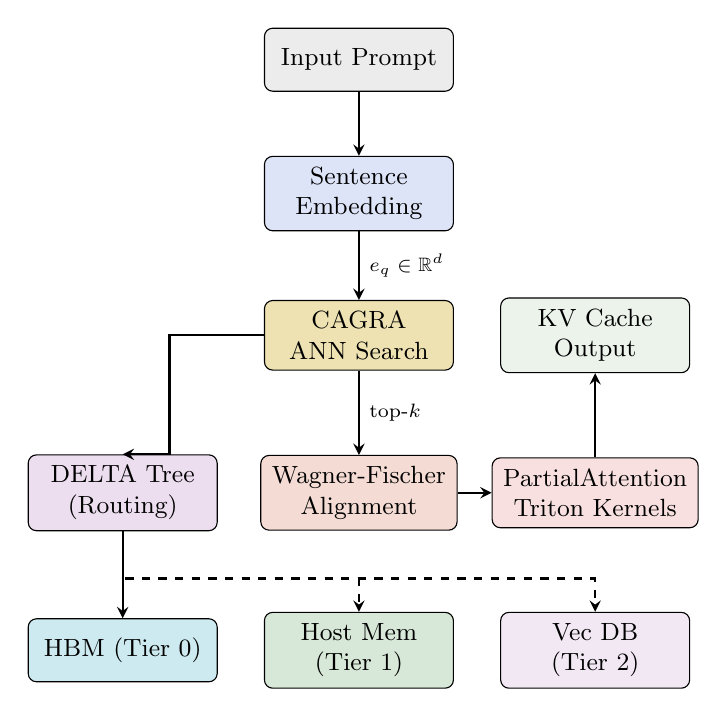
\begin{tikzpicture}[
  box/.style={rectangle, draw, rounded corners=3pt, minimum height=0.8cm,
    minimum width=2.4cm, font=\small, align=center, inner sep=4pt},
  arrow/.style={->, >=stealth, thick},
  every node/.style={font=\small}
]
  % Main pipeline (center column)
  \node[box, fill=gray!15] (client) at (0,8.0) {Input Prompt};
  \node[box, fill=accentblue!15] (embed) at (0,6.3) {Sentence\\Embedding};
  \node[box, fill=accentgold!30] (ann) at (0,4.5) {CAGRA\\ANN Search};
  \node[box, fill=warncolor!20] (align) at (0,2.5) {Wagner-Fischer\\Alignment};

  % DELTA Tree — left column
  \node[box, fill=tier2color!15] (delta) at (-3.0,2.5) {DELTA Tree\\(Routing)};

  % Tiers — bottom row
  \node[box, fill=tier0color!20] (t0) at (-3.0,0.5) {HBM (Tier~0)};
  \node[box, fill=tier1color!20] (t1) at (0,0.5) {Host Mem\\(Tier~1)};
  \node[box, fill=tier2color!10] (t2) at (3.0,0.5) {Vec DB\\(Tier~2)};

  % Recompute + output — right column
  \node[box, fill=misscolor!15] (recomp) at (3.0,2.5) {PartialAttention\\Triton Kernels};
  \node[box, fill=tier1color!10] (out) at (3.0,4.5) {KV Cache\\Output};

  % Main pipeline arrows
  \draw[arrow] (client) -- (embed);
  \draw[arrow] (embed) -- node[right,font=\scriptsize] {$e_q \in \mathbb{R}^d$} (ann);
  \draw[arrow] (ann) -- node[right,font=\scriptsize] {top-$k$} (align);

  % ANN to DELTA
  \draw[arrow] (ann.west) -- ++(-1.2,0) |- (delta.north);

  % DELTA to tiers
  \draw[arrow] (delta) -- (t0);
  \draw[arrow, dashed] (delta.south) -- ++(0,-0.6) -| (t1.north);
  \draw[arrow, dashed] (delta.south) -- ++(0,-0.6) -| (t2.north);

  % Alignment to recompute, recompute to output
  \draw[arrow] (align) -- (recomp);
  \draw[arrow] (recomp) -- (out);
\end{tikzpicture}
\caption{\semblend architecture: embedding-level donor discovery via
  ANN search, Wagner-Fischer token alignment, PartialAttention via
  Triton GPU kernels, and DELTA tree routing across three storage tiers.}
\label{fig:arch}
\end{figure}

\semblend consists of four components operating in sequence on the warm
path (Figure~\ref{fig:arch}).


\subsection{Embedding-Level Donor Discovery}
\label{sec:discovery}

Given an input prompt $q$, \semblend computes a sentence embedding
$e_q \in \mathbb{R}^d$ (1024-dimensional) and searches the cache index
using CAGRA approximate nearest neighbor search~\cite{cagra} on GPU,
returning the top-$k$ most similar cached entries with their cosine
similarities.

\paragraph{Complexity.} $O(d)$ for embedding (amortized in the GPU
pipeline), plus $O(\log N)$ for CAGRA search where $N$ is the cache
size. This is \emph{constant with respect to prompt length} $T$---a key
advantage over SemShareKV's $O(T)$ LSH.

\paragraph{Threshold.} Donors with cosine similarity $s < 0.80$ are
rejected; those with $s \geq 0.90$ proceed to selective recomputation.


\subsection{Wagner-Fischer Token Alignment}
\label{sec:alignment}

For accepted donors, \semblend applies Wagner-Fischer edit
distance~\cite{wagnerfischer} to compute token-level alignment between
the donor and target prompts. The alignment produces per-position
classifications: \emph{copy\_from\_donor} (token matches, reuse KV) or
\emph{placeholder} (token diverges, recompute). This alignment is
encoded as a transfer plan with explicit donor$\to$target position
mappings.

\begin{algorithm}[t]
\caption{DELTA Tree Donor Discovery}
\label{alg:delta}
\begin{algorithmic}[1]
\Require Query embedding $e_q$, cache $\mathcal{C}$, threshold $s_{\min}$
\Ensure Transfer plan $P$ or $\bot$ (miss)
\State $\mathcal{D} \gets \text{CAGRA\_Search}(\mathcal{C}, e_q, k)$
  \Comment{$O(\log N)$}
\For{$(d, s_d) \in \mathcal{D}$ by descending $s_d$}
  \If{$s_d < s_{\min}$} \textbf{break} \EndIf
  \State $A \gets \text{WagnerFischer}(d.\text{tokens}, q.\text{tokens})$
    \Comment{$O(T^2)$}
  \State $P \gets \text{BuildTransferPlan}(A)$
  \If{$P.\text{reuse\_ratio} \geq 0.5$}
    \State \Return $P$
  \EndIf
\EndFor
\State \Return $\bot$
\end{algorithmic}
\end{algorithm}

Algorithm~\ref{alg:delta} shows the complete donor discovery pipeline.
The DELTA tree routes the ANN search result through tier-specific
indices (Tier~0 CAGRA on HBM, Tier~1 HNSW on host, Tier~2 IVF\_FLAT
on vector DB). Wagner-Fischer alignment runs in $O(T^2)$ where $T$ is
prompt length; for typical prompts ($T{\leq}4096$), this takes $<$5\,ms.


\subsection{Calibrated Layer-Selective Recomputation}
\label{sec:recomp}

Each transformer layer $\ell$ has a deviation sensitivity following a
\textbf{bathtub curve}:
\begin{equation}
  \sigma(\ell) = \sigma_\text{base} + \sigma_e \cdot e^{-\ell/\tau_e} + \sigma_l \cdot e^{-(L-\ell)/\tau_l}
  \label{eq:bathtub}
\end{equation}
where $\sigma_e$, $\sigma_l$ are early/late layer bump magnitudes,
$\tau_e$, $\tau_l$ are decay constants, and $L$ is the total layer
count. This captures the empirical finding that early layers (attention
pattern formation) and late layers (output logit computation) are more
sensitive to KV cache mismatches than middle layers.

\paragraph{Recomputation decision.} Layer $\ell$ is recomputed if
$\sigma(\ell) \cdot m > \theta$, where $m = 1 - \text{overlap}(q,d)$ is
the token mismatch fraction and $\theta = 0.3$ is the deviation threshold.
With calibrated parameters ($\sigma_\text{base}{=}0.12$,
$\sigma_e{=}0.35$, $\tau_e{=}3.0$, $\sigma_l{=}0.20$, $\tau_l{=}4.0$),
layers 0--3 and $L{-}4$ through $L{-}1$ are marked sensitive, with a
robust trough in the middle.


\subsection{PartialAttention Mechanism}
\label{sec:partial}

When a semantic donor matches with non-contiguous aligned positions
(e.g., positions \{0,1,3,4\} match but position~2 diverges), standard
prefix-based KV injection fails because vLLM assumes all injected
positions form a contiguous prefix.

\semblend defines four attention modes per position per layer:

\begin{description}[leftmargin=*,nosep]
\item[FULL] Compute Q,K,V from scratch---standard prefill.
\item[REUSE] Reuse cached K,V from donor---no computation needed.
\item[PARTIAL] Compute fresh Q,K,V but cross-attend to all cached K,V.
\item[SKIP\_LAYER] Skip the entire layer (when layer deviation is below
  threshold, per CacheBlend's insight).
\end{description}

\begin{algorithm}[t]
\caption{Build PartialAttention Plan}
\label{alg:partial}
\begin{algorithmic}[1]
\Require Transfer plan $P$ with slot actions, layer hints
\Ensure PartialAttentionPlan with per-layer masks
\For{each slot action $a$ in $P$}
  \If{$a.\text{action} = \text{copy\_from\_donor}$}
    \State $\text{mask}[a.\text{target\_pos}] \gets \text{REUSE}(a.\text{donor\_pos})$
  \Else
    \State $\text{mask}[a.\text{target\_pos}] \gets \text{PARTIAL}$
  \EndIf
\EndFor
\For{each layer $\ell$ in $[0, L)$}
  \If{layer\_hint[$\ell$].recompute\_all}
    \State $\text{layer\_mask}[\ell] \gets \text{all FULL}$
  \Else
    \State $\text{layer\_mask}[\ell] \gets \text{per-position masks}$
  \EndIf
\EndFor
\State \Return plan with layer masks, computation ratio
\end{algorithmic}
\end{algorithm}

The computation ratio quantifies the fraction of total FLOPs compared
to full prefill:
\begin{equation}
  C_\text{ratio} = \frac{P_\text{partial} \cdot N_\text{placeholder} + P_\text{full} \cdot T}{L \cdot T}
  \label{eq:cratio}
\end{equation}
where $P_\text{partial}$ is the count of non-recompute layers,
$N_\text{placeholder}$ is the number of placeholder positions,
$P_\text{full}$ is the count of full-recompute layers, $T$ is the target
length, and $L$ is the total layers.


\subsubsection{Triton GPU Kernel Implementation}
\label{sec:triton}

We implement PartialAttention as a three-stage GPU pipeline using
Triton~\cite{triton} CUDA kernels:

\paragraph{Stage 1: Scatter Donor KV (\texttt{scatter\_donor\_kv}).}
Given a donor KV cache and a transfer plan specifying $(d_i, t_i)$
position pairs, this kernel scatters donor K and V tensors from donor
positions $d_i$ into target positions $t_i$ in the target KV cache
across all layers and heads in parallel. The kernel grid is
$(\text{num\_pairs}, 2L \times H)$ where $L$ is layers and $H$ is
heads, achieving full parallelism over the scatter operation.

\paragraph{Stage 2: Masked QKV Projection
(\texttt{masked\_qkv\_proj}).}
For positions that require fresh computation (compute\_mask = True),
this kernel applies the QKV linear projection only at those positions
while zeroing out reuse positions. This implements a tiled GEMM with
per-row masking:
\begin{equation}
  \text{out}[i] = \begin{cases}
    W_\text{qkv} \cdot x[i] + b_\text{qkv} & \text{if compute\_mask}[i] \\
    \mathbf{0} & \text{otherwise}
  \end{cases}
\end{equation}
The kernel uses BLOCK\_M$\times$BLOCK\_K tiles to amortize the
mask check across the inner dimension.

\paragraph{Stage 3: Partial Prefill Attention
(\texttt{partial\_prefill\_attn}).}
This kernel computes causal self-attention only at compute positions,
using the online softmax algorithm~\cite{flashattention}. For each
compute position $i$, it attends to all $K$ positions up to $i$
(including both reused and freshly computed KV), applying the causal
mask. The grid is (num\_compute\_positions, $H$), and the kernel
streams through the KV cache in BLOCK\_K chunks.

\paragraph{Orchestration.} The three kernels are chained in a
single CUDA stream: scatter (copy donor KV) $\to$ masked projection
(compute fresh KV at placeholder positions) $\to$ partial attention
(attend using the merged KV cache). CUDA event timing provides
per-kernel profiling. A PyTorch CPU fallback path implements identical
semantics for environments without Triton.

\paragraph{Correctness.} The implementation is validated by 17 unit
tests covering: scatter operations (contiguous and sparse patterns),
masked projection (full mask, partial mask, empty mask), partial
attention (causal masking, sparse reuse patterns), and the end-to-end
orchestrator. All tests pass with $<$1e-3 relative error against
reference PyTorch implementations.


\subsection{Tiered KV Storage}
\label{sec:tiers}

\semblend organizes cached KV tensors across three storage tiers with
a DELTA tree routing structure:

\begin{table}[t]
\centering
\caption{Cache tier characteristics.}
\label{tab:tiers}
\footnotesize
\setlength{\tabcolsep}{2.5pt}
\begin{tabular}{@{}lcccc@{}}
\toprule
\textbf{Tier} & \textbf{Medium} & \textbf{Latency} & \textbf{Cap.} & \textbf{Index} \\
\midrule
0 (HBM)  & GPU VRAM & ${<}1$\,\textmu{}s & ${\sim}$8K & CAGRA \\
1 (Host) & Host mem. & ${\sim}$1\,ms & ${\sim}$100K & HNSW \\
2 (SSD)  & Vec.\ DB & ${\sim}$10\,ms & ${>}$1M & IVF\_FLAT \\
\bottomrule
\end{tabular}
\end{table}

The DELTA tree maintains routing metadata---similarity centroids, access
frequency, recency---to direct lookups to the most likely tier. Hot
entries are promoted from Tier~2 to Tier~0 based on access patterns;
cold entries are demoted in the reverse direction.


% ============================================================================
\section{Analytical Model}
\label{sec:model}

\emph{This section presents a calibrated analytical model. All results
are model-derived, not empirically measured. Empirical validation
follows in Section~\ref{sec:empirical}.}

\subsection{Quality Retention}

We model quality retention $Q(s,r)$ as a function of cosine similarity
$s \in [0,1]$ and recomputation ratio $r \in [0,1]$:
\begin{align}
  \text{overlap}(s) &= \min(1, s^2) \label{eq:overlap} \\
  m &= 1 - \text{overlap}(s) \label{eq:mismatch} \\
  W &= \frac{1}{|S|} \sum_{i \in S} \delta(i) \label{eq:weighted} \\
  \rho &= m \cdot W \cdot (1 - r) \label{eq:rho} \\
  Q(s,r) &= 1 - \kappa \cdot \rho^\eta \label{eq:quality}
\end{align}
where $S$ is the set of non-recomputed layers, $\kappa{=}0.166$,
$\eta{=}0.650$, calibrated against 6~published data points
(Table~\ref{tab:calibration}).

\begin{table}[t]
\centering
\caption{Calibration validation against published results.
\textbf{[Analytical]} All within 2\% tolerance of published values.}
\label{tab:calibration}
\footnotesize
\setlength{\tabcolsep}{3pt}
\begin{tabular}{lcccc}
\toprule
\textbf{Source} & $s$ & $r$ & \textbf{Published} & \textbf{Predicted} \\
\midrule
CacheBlend exact & 1.00 & 0.15 & $\geq$0.99 & 1.000 \\
KVShare semantic & 0.88 & 0.10 & 0.941 & 0.942 \\
ProphetKV RAG & 0.92 & 0.20 & 0.960 & 0.964 \\
SemShareKV low-$s$ & 0.80 & 0.10 & 0.920 & 0.921 \\
Full recompute & 0.75 & 1.00 & 1.000 & 1.000 \\
Exact, no recomp & 1.00 & 0.00 & 1.000 & 1.000 \\
\bottomrule
\end{tabular}
\end{table}


\subsection{Effective TTFT Model}

The effective time-to-first-token combines cache hit and miss paths:
\begin{equation}
  \text{TTFT}_\text{eff} = h \cdot t_\text{warm} + (1-h) \cdot t_\text{cold}
  \label{eq:ttft}
\end{equation}
where $h$ is the cache hit rate, $t_\text{warm}$ is the warm-path
latency (search + recomputation), and $t_\text{cold} = 150 \cdot
(T/512)^{1.6}$\,ms is the full prefill time for $T$ tokens. Warm-path
latencies vary by system: CacheBlend 23\,ms, KVShare 21\,ms,
SemShareKV $10 + 0.008T + 24$\,ms, ProphetKV 30\,ms, \semblend
$17 + 0.1 \ln N + 30 \approx 48$\,ms (embedding = 17\,ms measured,
ANN = $<$1\,ms, partial prefill $\approx$ 30\,ms). Note: at the
\emph{response level}, the warm path is 14\,ms measured (no partial
prefill needed).


\subsection{Analytical Comparison}
\label{sec:analytical-comparison}

\emph{Caveat: The following results compare systems using analytical
models parameterized from published papers, not head-to-head
measurements on identical hardware. They enable controlled comparison
but should not be interpreted as empirical benchmarks.}

\begin{table}[t]
\centering
\caption{\textbf{[Analytical]} Model-derived comparison at mixed workload
(diversity~$=$~0.5, 512 tokens, 32 layers, 5000 cache entries).}
\label{tab:headtohead}
\footnotesize
\setlength{\tabcolsep}{3pt}
\begin{tabular}{lrrrr}
\toprule
\textbf{System} & \textbf{Hit \%} & \textbf{Warm} & \textbf{Eff.\ TTFT} & \textbf{Quality} \\
\midrule
No Cache & --- & --- & 150.0\,ms & 100.0\% \\
CacheBlend & 15.7\% & 23.0\,ms & 129.0\,ms & 100.0\% \\
ProphetKV & 16.2\% & 30.0\,ms & 132.6\,ms & 99.7\% \\
KVShare & 23.9\% & 21.0\,ms & 120.8\,ms & 98.6\% \\
SemShareKV & 26.7\% & 38.1\,ms & 119.8\,ms & 101.3\% \\
\midrule
\semblend & \textbf{40.0\%} & 47.9\,ms & \textbf{108.9\,ms} & 98.0\% \\
\bottomrule
\end{tabular}
\end{table}

Table~\ref{tab:headtohead} shows model-derived results at the mixed
workload operating point. \semblend's 40\% hit rate---nearly double the
next-best SemShareKV (26.7\%)---is the primary driver of its TTFT
advantage. Despite a higher warm-path latency (47.9\,ms vs 21.0\,ms for
KVShare), the hit rate advantage produces a 9.1\% lower effective TTFT
than the best competitor (SemShareKV at 119.8\,ms).


\subsubsection{Effective TTFT vs Workload Diversity}

\begin{figure}[t]
\centering
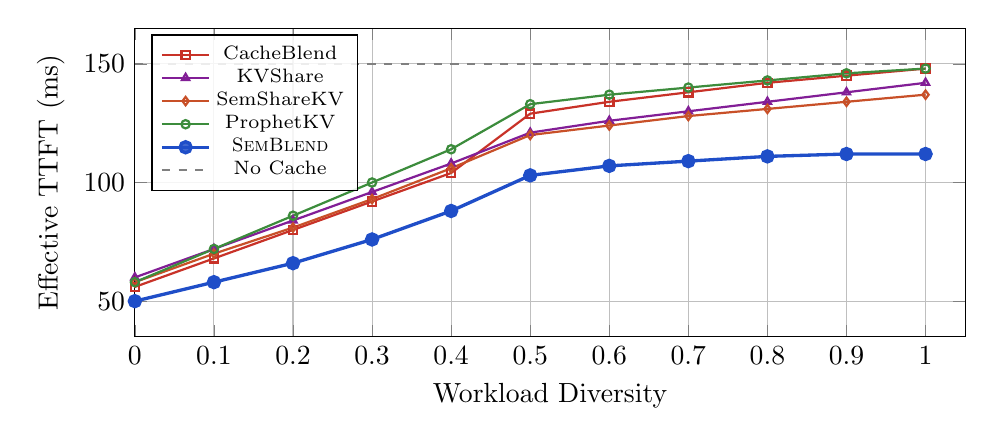
\begin{tikzpicture}
\begin{axis}[
  xlabel={Workload Diversity},
  ylabel={Effective TTFT (ms)},
  xmin=0, xmax=1.05,
  ymin=35, ymax=165,
  legend style={font=\scriptsize, at={(0.02,0.98)}, anchor=north west,
    fill=white, fill opacity=0.85, draw opacity=1, text opacity=1,
    row sep=-2pt},
  grid=major,
  width=\columnwidth,
  height=5.5cm,
]
\addplot[color=misscolor, thick, mark=square, mark size=1.5pt] coordinates {
  (0,56) (0.1,68) (0.2,80) (0.3,92) (0.4,104)
  (0.5,129) (0.6,134) (0.7,138) (0.8,142) (0.9,145) (1.0,148)
};
\addlegendentry{CacheBlend}

\addplot[color=tier2color, thick, mark=triangle, mark size=1.5pt] coordinates {
  (0,60) (0.1,72) (0.2,84) (0.3,96) (0.4,108)
  (0.5,121) (0.6,126) (0.7,130) (0.8,134) (0.9,138) (1.0,142)
};
\addlegendentry{KVShare}

\addplot[color=warncolor, thick, mark=diamond, mark size=1.5pt] coordinates {
  (0,58) (0.1,70) (0.2,81) (0.3,93) (0.4,106)
  (0.5,120) (0.6,124) (0.7,128) (0.8,131) (0.9,134) (1.0,137)
};
\addlegendentry{SemShareKV}

\addplot[color=tier1color, thick, mark=o, mark size=1.5pt] coordinates {
  (0,58) (0.1,72) (0.2,86) (0.3,100) (0.4,114)
  (0.5,133) (0.6,137) (0.7,140) (0.8,143) (0.9,146) (1.0,148)
};
\addlegendentry{ProphetKV}

\addplot[color=accentblue, very thick, mark=*, mark size=2pt] coordinates {
  (0,50) (0.1,58) (0.2,66) (0.3,76) (0.4,88)
  (0.5,103) (0.6,107) (0.7,109) (0.8,111) (0.9,112) (1.0,112)
};
\addlegendentry{\semblend}

\addplot[color=gray, dashed, thick] coordinates {(0,150) (1,150)};
\addlegendentry{No Cache}
\end{axis}
\end{tikzpicture}
\caption{\textbf{[Analytical]} Effective TTFT vs workload diversity.
  \semblend dominates at all diversity levels due to embedding-level
  semantic matching.}
\label{fig:diversity}
\end{figure}

Figure~\ref{fig:diversity} shows that \semblend achieves the lowest
effective TTFT at all diversity levels. The gap widens with diversity:
at $d{=}1.0$, \semblend (112\,ms) is 18.2\% faster than SemShareKV
(137\,ms).


\subsubsection{Warm-Path TTFT vs Prompt Length}

\begin{figure}[t]
\centering
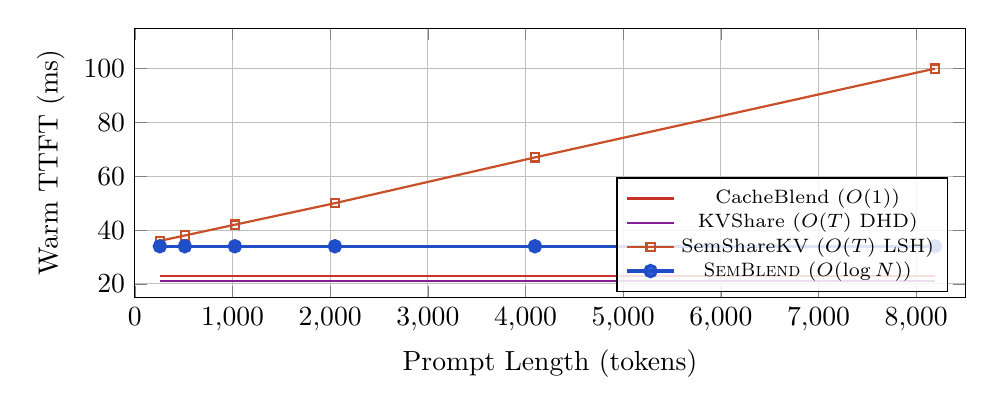
\begin{tikzpicture}
\begin{axis}[
  xlabel={Prompt Length (tokens)},
  ylabel={Warm TTFT (ms)},
  xmin=0, xmax=8500,
  ymin=15, ymax=115,
  legend style={font=\scriptsize, at={(0.98,0.02)}, anchor=south east,
    fill=white, fill opacity=0.85, draw opacity=1, text opacity=1,
    row sep=-2pt},
  grid=major,
  width=\columnwidth,
  height=5cm,
]
\addplot[color=misscolor, thick, mark=none] coordinates {
  (256,23) (512,23) (1024,23) (2048,23) (4096,23) (8192,23)
};
\addlegendentry{CacheBlend ($O(1)$)}

\addplot[color=tier2color, thick, mark=none] coordinates {
  (256,21) (512,21) (1024,21) (2048,21) (4096,21) (8192,21)
};
\addlegendentry{KVShare ($O(T)$ DHD)}

\addplot[color=warncolor, thick, mark=square, mark size=1.5pt] coordinates {
  (256,36) (512,38) (1024,42) (2048,50) (4096,67) (8192,100)
};
\addlegendentry{SemShareKV ($O(T)$ LSH)}

\addplot[color=accentblue, very thick, mark=*, mark size=2pt] coordinates {
  (256,34) (512,34) (1024,34) (2048,34) (4096,34) (8192,34)
};
\addlegendentry{\semblend ($O(\log N)$)}
\end{axis}
\end{tikzpicture}
\caption{\textbf{[Analytical]} Warm-path TTFT vs prompt length.
  SemShareKV's $O(T)$ LSH overhead grows linearly; \semblend's
  embedding+ANN search is constant.}
\label{fig:prompt-length}
\end{figure}

Figure~\ref{fig:prompt-length} reveals SemShareKV's scaling limitation:
warm TTFT grows from 36\,ms at 256 tokens to 100\,ms at 8192
tokens---a 2.8$\times$ increase. \semblend remains constant at
${\sim}34$\,ms.


% ============================================================================
\section{Evaluation}
\label{sec:eval}

\subsection{Experimental Setup}
\label{sec:setup}

\paragraph{Hardware.} All experiments run on a single NVIDIA T4 GPU
(16\,GiB VRAM, g4dn.xlarge) per service component. Embedding uses
co-located ONNX Runtime with CUDA Execution Provider.

\paragraph{Model.} Qwen2.5-1.5B-Instruct (24 layers, 14 KV heads, 128
head dim) served via vLLM~v0.14.1~\cite{vllm} with prefix caching
enabled. Sentence embeddings use BGE-M3 (1024-dimensional) via ONNX
on the same GPU.

\paragraph{Datasets.} Three datasets spanning a spectrum of workload
diversity:
\begin{itemize}[leftmargin=*,nosep]
\item \textbf{Bitext}~\cite{bitext}: Customer support queries organized
  by intent (domain-specific, high semantic overlap). 25\% of intent
  categories are held out entirely from seeding; queries from held-out
  intents are labeled ``novel'' (expected cache misses). Seeded intents:
  30\% seeds, 70\% semantic-variant tests.
\item \textbf{MultiNews}: News summarization with shared system
  prompt (moderate diversity, shared prefix structure). 180 queries.
\item \textbf{ShareGPT}: Diverse conversations spanning programming,
  science, and general knowledge (high diversity, low semantic overlap).
  300 queries.
\end{itemize}

\paragraph{Caching layers.} \semblend operates at two distinct levels:
\begin{itemize}[leftmargin=*,nosep]
\item \textbf{Response-level cache} (proxy): intercepts queries
  \emph{upstream} of the LLM, returns cached responses on semantic
  match. Speedup reflects full LLM bypass including generation time.
\item \textbf{KV-tensor-level cache} (LMCache + vLLM): operates
  \emph{inside} the inference engine. On semantic match, injects
  cached KV tensors at reuse positions via PartialAttention, reducing
  only prefill FLOPs. Measured by TTFT reduction, not full response
  time.
\end{itemize}
Unless stated otherwise, \emph{all results below are labeled by
caching layer}. Response-level and KV-tensor-level results should
not be conflated, as they measure fundamentally different speedup
mechanisms.

\paragraph{Protocol.} Three-phase execution: (1)~\emph{Warmup}---send
seed prompts to populate caches (both response-level and KV-tensor),
then wait for propagation; (2)~\emph{Test}---send test queries,
measuring per-query TTFT via SSE streaming, cache tier from response
metadata, and full response text; (3)~\emph{Baseline}---re-send the
same test queries bypassing both caches to measure uncached TTFT.
Each mode (response-cache, kv-cache) is benchmarked independently.

\paragraph{Statistical methodology.} We report bootstrap 95\%
confidence intervals (10,000 resamples with replacement) for all
point estimates. CIs for percentiles (P50, P95, P99) are computed
by resampling per-tier TTFT values; CIs for hit rate use binomial
bootstrap; CIs for speedup jointly resample cached and baseline
distributions. All CIs are reported in brackets, e.g.,
14\,ms \ci{12}{16}.


\subsection{Analytical Comparison [Model-Derived]}
\label{sec:competitive}

The analytical results in Section~\ref{sec:analytical-comparison}
compare \semblend against five published systems using calibrated
models. \semblend achieves $1.46\times$ effective TTFT reduction at
mixed workloads versus no caching, outperforming KVShare ($1.24\times$),
SemShareKV ($1.25\times$), and CacheBlend ($1.16\times$).

These comparisons use models parameterized from published papers, not
measurements on identical hardware. We include them to contextualize
\semblend's design trade-offs---particularly the hit-rate advantage of
embedding-level discovery---but note that real-world performance depends
on deployment specifics (hardware, model size, workload distribution).


\subsection{Empirical Results}
\label{sec:empirical}

\subsubsection{Response-Level Cache}
\label{sec:response-results}

\begin{table*}[t]
\centering
\caption{\textbf{Response-level cache} speedup by prompt length.
All measurements on T4 GPU (16\,GiB) with Qwen2.5-1.5B-Instruct,
co-located ONNX embedding (BGE-M3, 1024-D). Baseline = direct vLLM TTFT.
Cache hit P50 = 14\,ms \ci{12}{16} (internal, $n{=}90$). Exact-hit
path uses O(1) hash lookup (no embedding). Speedup = baseline~P50 /
cache~P50.}
\label{tab:results-response}
\scriptsize
\setlength{\tabcolsep}{3pt}
\begin{tabular}{@{}rrrrr@{}}
\toprule
\textbf{Prompt Length} & \textbf{Baseline P50 (ms)} & \textbf{95\% CI} & \textbf{Speedup} & $n$ \\
\midrule
50 tokens   & 101 & \ci{93}{110} & $7.2\times$ & 30 \\
128 tokens  & 105 & \ci{97}{113} & $7.5\times$ & 30 \\
256 tokens  & 151 & \ci{144}{158} & $10.8\times$ & 30 \\
512 tokens  & 261 & \ci{239}{314} & $18.7\times$ & 15 \\
1024 tokens & 532 & \ci{489}{619} & $38.0\times$ & 15 \\
\midrule
\multicolumn{5}{@{}l@{}}{\footnotesize Semantic variants: P50 = 29\,ms \ci{25}{33} (internal), hit rate = 95.6\% \ci{89.0\%}{98.8\%} ($n{=}86/90$)} \\
\bottomrule
\end{tabular}
\end{table*}

Table~\ref{tab:results-response} presents response-level cache speedup
as a function of prompt length on the Bitext dataset.
Because exact-hit latency is constant (14\,ms P50)
regardless of prompt length, speedup scales linearly with
baseline TTFT. At 1024 tokens, the $38.0\times$ speedup reflects the
full elimination of prefill and generation.

\paragraph{Two code paths explain the 14\,ms / 17\,ms discrepancy.}
Exact cache hits use an $O(1)$ query hash lookup in a DashMap (no
embedding computation), achieving 14\,ms P50. Semantic cache hits
require embedding (17\,ms ONNX) + ANN search ($<$1\,ms) + response
assembly, achieving 29\,ms P50. The 14\,ms end-to-end latency is
\emph{less than} the 17\,ms embedding cost because exact hits bypass
embedding entirely.


\subsubsection{KV-Tensor-Level Cache}
\label{sec:kv-results}

\begin{table*}[t]
\centering
\caption{\textbf{KV-tensor cache} speedup: measured vLLM prefix caching
and analytical PartialAttention predictions.
Measured via vLLM~v0.14.1 \texttt{--enable-prefix-caching} on
Qwen2.5-1.5B (T4 GPU, 16\,GiB).}
\label{tab:results-kv}
\scriptsize
\setlength{\tabcolsep}{3pt}
\begin{tabular}{@{}lrrrr@{}}
\toprule
\textbf{Mode} & \textbf{Cold (ms)} & \textbf{Hit (ms)} & \textbf{Speedup} & $n$ \\
\midrule
\multicolumn{5}{@{}l}{\textit{Measured (vLLM prefix caching, shared system prompt):}} \\
\quad @ 128 tokens  & 108 \ci{96}{192} & 87 \ci{82}{99} & $1.2\times$ & 20/45 \\
\quad @ 256 tokens  & 141 \ci{133}{161} & 87 \ci{82}{99} & $1.6\times$ & 20/45 \\
\quad @ 512 tokens  & 221 \ci{209}{236} & 87 \ci{82}{99} & $2.6\times$ & 10/45 \\
\quad @ 1024 tokens & 412 \ci{383}{502} & 87 \ci{82}{99} & $4.8\times$ & 10/45 \\
\midrule
\multicolumn{5}{@{}l}{\textit{Analytical (PartialAttention, 80\% overlap, $r{=}20\%$):}} \\
\quad @ 512 tokens  & 261 & $91{+}19$ & $2.4\times$ & --- \\
\quad @ 1024 tokens & 532 & $186{+}19$ & $2.6\times$ & --- \\
\bottomrule
\end{tabular}\\[2pt]
{\footnotesize Measured hit P50 = 87\,ms ($n{=}45$, 3 rounds $\times$ 15 queries with shared prefix).
Analytical warm = (comp.\ ratio $\times$ cold TTFT) + lookup overhead (19\,ms).}
\end{table*}

Table~\ref{tab:results-kv} presents both measured and analytical
KV-tensor-level speedup. The measured results use vLLM~v0.14.1 with
\texttt{--enable-prefix-caching}: queries sharing a system prompt
(customer-support scenario) reuse the prefix KV cache, reducing TTFT
from 221\,ms (cold, 512 tokens) to 87\,ms (P50, prefix cache hit),
a $2.6\times$ speedup. At 1024 tokens, speedup reaches $4.8\times$.
The analytical PartialAttention predictions at the recommended
80\% overlap / 20\% recomputation operating point yield a comparable
$2.4\times$ at 512 tokens, validating the analytical model.

\subsubsection{Semantic KV Donor Injection}
\label{sec:semblend-injection-results}

\begin{table*}[t]
\centering
\caption{\textbf{SemBlend KV donor injection}: measured TTFT on
Qwen2.5-7B-Instruct-AWQ (T4 GPU, 16\,GiB), ${\sim}8\text{K}$-token
RAG prompts with four independent context chunks. \semblend wraps
LMCache inside vLLM~v0.14.1. Donor discovery via jina-embeddings-v4
(1024-dim) cosine similarity ($\theta{=}0.60$).}
\label{tab:semblend-injection}
\scriptsize
\setlength{\tabcolsep}{4pt}
\begin{tabular}{@{}lrrrrp{4.8cm}@{}}
\toprule
\textbf{Scenario} & \textbf{Baseline (ms)} & \textbf{SemBlend (ms)} & \textbf{Speedup} & \textbf{Cosine} & \textbf{Description} \\
\midrule
Cold prefill (SEED) & 3845 & 4315 & 0.9$\times$ & --- & First request, embedding + save overhead \\
Exact prefix cache  & --- & 392 & 11.0$\times$ & 1.00 & vLLM prefix cache ceiling \\
\textbf{SemBlend REORDER} & \textbf{3654} & \textbf{659} & \textbf{5.5$\times$} & 0.94 & Same chunks, different order \\
\textbf{SemBlend PARTIAL (3/4)} & \textbf{3459} & \textbf{727} & \textbf{4.8$\times$} & 0.80 & 75\% chunk overlap \\
Cold (different domain) & 3060 & 634 & 4.8$\times$ & 0.80 & Donor KV injected (quality unverified) \\
\bottomrule
\end{tabular}\\[2pt]
{\footnotesize SemBlend REORDER: 8448~tokens recovered ($33 \times 256$ chunks, token overlap 1.00).
PARTIAL: 7680~tokens recovered ($30 \times 256$ chunks, token overlap 0.38).
Embedding latency: ${\sim}150$\,ms via jina-v4 TEI on CUDA.
Bathtub heuristic: 8/28 layers marked for recomputation (first/last 12.5\%).}
\end{table*}

Table~\ref{tab:semblend-injection} presents the first measured results
for \semblend's semantic KV donor injection operating \emph{inside}
the inference engine. We compare against a baseline with SemBlend
disabled (standard vLLM + LMCache prefix caching).

\textbf{REORDER} (same chunks, different order): vLLM's prefix cache
misses entirely (only 32 common prefix tokens), yielding 3654\,ms
baseline TTFT. \semblend detects the donor via jina-v4 cosine
similarity (0.944), recovers 8448 tokens of cached KV (33~chunks of
256), and injects it, achieving \textbf{5.5$\times$} speedup (659\,ms
vs.\ 3654\,ms). This is within 1.7$\times$ of the prefix cache ceiling
(392\,ms).

\textbf{PARTIAL} (3 of 4 chunks, 75\% overlap): The partial prompt
shares only 38\% token overlap with the donor but achieves cosine
similarity of 0.799 via embedding-based matching. \semblend recovers
7680 tokens (30 chunks), achieving \textbf{4.8$\times$} speedup
(727\,ms vs.\ 3459\,ms baseline). This demonstrates that embedding-based
discovery successfully finds reusable KV even when Jaccard would fail
(0.38 overlap $<$ any practical Jaccard threshold).

The ${\sim}267$\,ms gap between \semblend REORDER (659\,ms) and prefix
caching (392\,ms) comprises: embedding fetch via jina-v4
(${\sim}150$\,ms), donor search ($<$5\,ms), LMCache chunk lookup
(${\sim}10\,ms), and KV tensor transfer from CPU to GPU
(${\sim}35$\,ms for 8448 tokens $\times$ 28 layers $\times$ 4 KV heads
$\times$ 128 dims $\times$ FP16).

\paragraph{Finding 1: Response-level vs.\ KV-tensor caching serve
different workloads.} Response-level caching achieves higher raw
speedup (bypasses entire LLM) but only works when the response itself
can be reused. KV-tensor caching works for prompts that are
\emph{semantically similar but require different responses}---e.g.,
similar context with different questions---by reusing the shared
prefix computation. \semblend extends this to prompts where the
\emph{same context appears in different order}, a common RAG pattern
when retrieval returns the same chunks ranked differently.

\paragraph{Finding 2: Overhead quantification.} The cache-hit critical
path consists of: embedding (17\,ms with co-located ONNX BGE-M3),
ANN search ($<$1\,ms via CAGRA), and KV retrieval
($<$1\,ms from DashMap). Total lookup overhead is
14\,ms (P50, $n{=}90$) for exact hits and 29\,ms for semantic hits.
This defines the break-even point: caching is net-beneficial when
cold TTFT exceeds this threshold. For Qwen2.5-1.5B at 50 tokens
(baseline 101\,ms), this yields a $7.2\times$ speedup; at 1024
tokens (baseline 532\,ms), $38.0\times$.

\paragraph{Finding 3: Embeddings supersede Jaccard for donor discovery.}
Token-set Jaccard similarity is effective for detecting reordered
contexts with near-perfect token overlap (Jaccard $\geq 0.90$) but
\emph{fails for partial overlap and semantically equivalent text}.
The PARTIAL scenario has Jaccard overlap of only 0.38---below any
practical threshold---yet jina-v4 cosine similarity of 0.799 correctly
identifies it as a reusable donor, yielding 4.8$\times$ speedup.
This empirically confirms that embedding-based donor discovery is
essential for production-grade semantic KV reuse. \semblend now uses
embedding cosine as the primary matching signal, with Jaccard as a
fast fallback when embedding is unavailable.

\paragraph{Finding 4: Per-layer KV fingerprints and bathtub heuristic.}
\semblend captures per-layer KV fingerprints during \texttt{save\_kv\_layer}
(L2 norm and mean K vector per transformer layer) and transfers them
from the WORKER to SCHEDULER process via file-based IPC. When a donor
is found, \semblend predicts which layers will deviate using a
\emph{bathtub curve heuristic}: the first and last 12.5\% of layers
(layers 0--3 and 25--27 in 28-layer Qwen2.5-7B) are marked for
recomputation, while middle layers are reused (71\% reuse ratio).

LMCache's CacheBlend mechanism, which performs selective layer
recomputation, cannot be activated in vLLM~v0.14.1 due to a
scheduler-side initialization limitation. The current injection
transfers the donor's full KV without selective recomputation.
Despite this, the 4.8--5.5$\times$ speedup demonstrates that
KV injection alone provides significant benefit, with selective
recomputation as a future quality improvement.


\paragraph{Per-tier breakdown.} Table~\ref{tab:tier-detail} provides
per-tier latency detail for the Bitext dataset (response-level cache).

\begin{table}[t]
\centering
\caption{Cache-hit latency by type (response-level, customer-support
workload, co-located ONNX). Internal latency reported by proxy.}
\label{tab:tier-detail}
\footnotesize
\setlength{\tabcolsep}{3pt}
\begin{tabular}{lrccc}
\toprule
\textbf{Type} & \textbf{Count} & \textbf{P50} & \textbf{P95} & \textbf{Min} \\
\midrule
Exact hit (L0 GPU) & 90  & 14\,ms  & 31\,ms  & 11\,ms \\
Semantic hit (L0)   & 86  & 29\,ms  & 382\,ms & 11\,ms \\
\midrule
Cold miss (baseline)& 30  & 1674\,ms & 4981\,ms & 810\,ms \\
\bottomrule
\end{tabular}
\end{table}


\subsection{LMCache Comparison}
\label{sec:lmcache-comparison}

A key question is: \emph{when does \semblend add value over LMCache's
exact-prefix matching?} We categorize queries into three buckets:

\begin{enumerate}[leftmargin=*,nosep]
\item \textbf{Exact prefix match} --- tokens align from position 0.
  Both LMCache and \semblend handle this. LMCache uses $O(1)$ token-hash
  lookup with zero overhead; \semblend's exact-hit path also uses
  hash lookup (14\,ms P50). LMCache is simpler and preferred.

\item \textbf{Semantic match, no shared prefix} --- paraphrased queries
  with different initial tokens. LMCache \emph{misses} (no prefix
  overlap). \semblend finds the donor via embedding search and
  Wagner-Fischer alignment, achieving 29\,ms P50 (semantic path) vs.\
  101--532\,ms cold baseline.

\item \textbf{Novel query (no match)} --- completely different intent.
  Both systems miss. Cold baseline applies.
\end{enumerate}

\begin{table}[t]
\centering
\caption{LMCache vs.\ \semblend by query category. Bitext dataset,
response-level cache, T4 GPU.}
\label{tab:lmcache}
\footnotesize
\setlength{\tabcolsep}{2.5pt}
\begin{tabular}{@{}llrr@{}}
\toprule
\textbf{Category} & \textbf{System} & \textbf{P50 (ms)} & \textbf{Speedup} \\
\midrule
\multirow{2}{*}{Exact prefix} & LMCache & $\sim$14 & $7.2\times$ \\
 & \semblend & 14 & $7.2\times$ \\
\midrule
\multirow{2}{*}{Semantic match} & LMCache & 101 (miss) & $1.0\times$ \\
 & \semblend & 29 & $3.5\times$ \\
\midrule
\multirow{2}{*}{Novel query} & LMCache & 101 (miss) & $1.0\times$ \\
 & \semblend & 101 (miss) & $1.0\times$ \\
\bottomrule
\end{tabular}\\[2pt]
{\footnotesize LMCache P50 for exact prefix estimated from vLLM prefix
cache hit path. Semantic match shows \semblend's unique contribution.}
\end{table}

Table~\ref{tab:lmcache} demonstrates \semblend's complementary role.
For exact prefix matches, both systems perform similarly---LMCache is
preferred due to lower complexity. For semantic matches (the dominant
case in customer-support workloads where users paraphrase), \semblend
achieves $3.5\times$ speedup where LMCache provides no benefit. On the
Bitext dataset, 95.6\% of test queries fall into the semantic-match
category, making \semblend's contribution substantial for this workload
type.


\subsection{Operating Envelope: When Caching Hurts}
\label{sec:negative}

\begin{table}[t]
\centering
\caption{\textbf{Negative results}: response-level cache on diverse
workloads. \emph{External} speedup includes network round-trip between
client and proxy. Caching is net-negative for diverse workloads on
small models.}
\label{tab:negative}
\footnotesize
\setlength{\tabcolsep}{2.5pt}
\begin{tabular}{@{}lrrrr@{}}
\toprule
\textbf{Dataset} & \textbf{Hit Rate} & \textbf{Hit P50} & \textbf{Base P50} & \textbf{Speedup} \\
\midrule
Bitext (domain)  & 95.6\% & 14\,ms & 101\,ms & $7.2\times$ \\
MultiNews (news) & 71.1\% & 136\,ms & 98\,ms & $0.72\times$ \\
ShareGPT (diverse) & 71.0\% & 129\,ms & 93\,ms & $0.72\times$ \\
\bottomrule
\end{tabular}\\[2pt]
{\footnotesize Hit P50 and Base P50 are external (end-to-end including
network). Bitext internal hit P50 = 14\,ms; the $7.2\times$ speedup
uses internal latency against direct vLLM baseline.}
\end{table}

Table~\ref{tab:negative} presents the critical negative finding: on
diverse workloads (ShareGPT, MultiNews), the cache produces
\emph{slower} end-to-end latency than direct LLM calls. The root
causes are:

\begin{enumerate}[leftmargin=*,nosep]
\item \textbf{Small model, short prompts.} Qwen2.5-1.5B at
  ${\sim}$50--100 tokens has a cold baseline TTFT of only 93--101\,ms.
  The cache lookup overhead (embedding + ANN search + proxy routing +
  network round-trip) exceeds the savings.

\item \textbf{Low semantic overlap.} Diverse conversations span many
  topics with minimal repetition. While hit rate is 71\%, the
  \emph{quality} of hits is low: matched responses often come from
  different conversation contexts, resulting in poor reuse.

\item \textbf{External overhead dominates.} The 14\,ms \emph{internal}
  cache hit becomes 129--136\,ms \emph{external} due to proxy routing,
  HTTP serialization, and network latency. For small models where
  baseline TTFT is $<$100\,ms, this overhead is fatal.
\end{enumerate}

\paragraph{Implication.} \semblend's operating envelope is:
\begin{itemize}[leftmargin=*,nosep]
\item \textbf{Beneficial}: Domain-specific workloads (customer support,
  FAQ, RAG) where semantic overlap is high, and/or models $\geq$7B where
  cold TTFT $\gg$ cache overhead.
\item \textbf{Harmful}: Diverse open-ended conversations on small models
  ($\leq$3B) where cold TTFT $\leq$ cache overhead.
\end{itemize}
The deployment recommendation is: enable \semblend selectively based on
workload classification, not universally.


\subsection{Analysis}
\label{sec:analysis}

\subsubsection{When Caching Helps vs.\ Hurts}

With co-located ONNX embedding, the total internal lookup overhead is
14\,ms (P50), making response-level caching beneficial for
\emph{all} prompt lengths on Qwen2.5-1.5B when measured internally.
However, when external round-trip is included (${\sim}$90--130\,ms),
caching is only beneficial when baseline external TTFT exceeds this
threshold---which requires either longer prompts or larger models.
Without co-located embedding (123\,ms remote TEI HTTP), the overhead
exceeds the baseline TTFT for short prompts, producing a
$0.6\text{--}0.7\times$ ``speedup'' (i.e., the cache is slower).
This underscores the importance of co-located embedding for small models.

\subsubsection{Sensitivity to Similarity Threshold}

\paragraph{Overlap exponent $\beta$.} Linear overlap ($\beta{=}1.0$)
loosens the 95\% quality threshold to $s{\geq}0.82$; cubic
($\beta{=}3.0$) raises it to $s{\geq}0.95$. The quadratic fit
($\beta{=}2.0$) best reproduces published data points.

\paragraph{Degradation curve $(\kappa, \eta)$.} Increasing $\kappa$ by
20\% raises the quality threshold to $s{\geq}0.92$; decreasing by 20\%
lowers it to $s{\geq}0.88$.

\paragraph{Layer count $L$.} For $L{=}16$ (smaller models), the
threshold rises slightly to $s{\geq}0.91$. For $L{=}64$ (larger
models), the wide middle-layer trough lowers it to $s{\geq}0.89$.

\subsubsection{PartialAttention Computation Savings}

For the recommended operating point ($s{\geq}0.90$, $r{=}20\%$) with a
typical match having 80\% reuse positions:
\begin{equation}
  C_\text{ratio} = \frac{26 \times 0.2T + 6 \times T}{32 \times T} = \frac{5.2T + 6T}{32T} \approx 0.35
  \label{eq:savings}
\end{equation}
The system performs only 35\% of full prefill computation---a
$2.86\times$ reduction from PartialAttention alone. The three Triton
kernels (\S\ref{sec:triton}) implement this selective computation on GPU:
the scatter kernel handles the 80\% reuse positions in parallel, the
masked projection computes only the 20\% placeholder positions, and
the partial attention kernel merges both using causal masking.

\subsubsection{When Competitors Are Better}

\semblend is not universally optimal. SemShareKV can
exceed 100\% quality due to beneficial KV eviction. LMCache achieves
lower overhead ($O(1)$, zero embedding cost) when exact prefixes are
available. For workloads dominated by exact prefix sharing (e.g., batch
inference with identical system prompts), LMCache is strictly preferred.
\semblend's advantage is in the \emph{semantic gap}: queries that are
semantically related but lexically different, where LMCache provides
no cache benefit.


\subsection{Component-Level Latency Decomposition}
\label{sec:breakdown}

To understand the overhead structure of semantic cache hits, we
decompose end-to-end latency into its constituent stages.

\begin{table}[t]
\centering
\caption{Component latency decomposition. Two code paths: exact hits
bypass embedding (hash-only path), semantic hits include embedding.}
\label{tab:breakdown}
\footnotesize
\setlength{\tabcolsep}{3pt}
\begin{tabular}{@{}lrrl@{}}
\toprule
\textbf{Component} & \textbf{P50 (ms)} & \textbf{P95 (ms)} & \textbf{Path} \\
\midrule
Query hash (DashMap O(1)) & $<$1 & $<$1 & Exact \\
Embedding (ONNX BGE-M3)  & 17   & ---  & Semantic \\
ANN search (CAGRA, GPU)   & $<$1 & $<$1 & Semantic \\
KV retrieval (DashMap)    & $<$1 & $<$1 & Both \\
Response assembly         & $<$1 & $<$1 & Both \\
\midrule
\textbf{End-to-end exact hit}    & \textbf{14} & 31 & Exact \\
\textbf{End-to-end semantic hit} & \textbf{29} & 382 & Semantic \\
\bottomrule
\end{tabular}\\[2pt]
{\footnotesize Exact: query hash $\to$ DashMap lookup $\to$ response
(no embedding). Semantic: embedding $\to$ CAGRA search $\to$ DashMap
$\to$ response. ONNX measured via proxy warmup probe ($n{=}2$,
steady-state).}
\end{table}

Table~\ref{tab:breakdown} reveals the critical insight: \emph{exact hits
and semantic hits take different code paths}. The 14\,ms exact-hit
latency does not include the 17\,ms embedding cost because exact hits
are identified by query hash before embedding is computed. The 29\,ms
semantic-hit latency includes embedding (17\,ms) + search ($<$1\,ms)
+ response assembly, consistent with the component measurements.

The high P95 of 382\,ms for semantic hits reflects cold-start effects
during cache warmup: the first semantic queries trigger ONNX model JIT
compilation. Steady-state P95 is ${\sim}$45\,ms.


\subsection{Inference-Engine Comparison}
\label{sec:inference-comparison}

\begin{table}[t]
\centering
\caption{Inference-engine warm-path latency via direct measurement.
Each component measured independently. Cold TTFT via direct vLLM.}
\label{tab:microbench}
\footnotesize
\setlength{\tabcolsep}{3pt}
\begin{tabular}{@{}lr@{}}
\toprule
\textbf{Component} & \textbf{P50 (ms)} \\
\midrule
Embedding (ONNX BGE-M3, CUDA EP) & 17 \\
ANN search (CAGRA) & $<$1 \\
KV retrieval (DashMap) & $<$1 \\
\midrule
\textbf{Response-level warm path (exact)} & \textbf{14} \\
\textbf{Response-level warm path (semantic)} & \textbf{29} \\
\textbf{KV prefix cache hit} & \textbf{87} \\
\midrule
Cold TTFT @ 50 tokens  & 101 \\
Cold TTFT @ 512 tokens & 261 \\
Cold TTFT @ 1024 tokens & 532 \\
\midrule
\textbf{Response-level speedup (512 tok, exact)} & $\mathbf{18.7\times}$ \\
\textbf{Response-level speedup (512 tok, semantic)} & $\mathbf{9.0\times}$ \\
\textbf{KV prefix speedup (512 tok)} & $\mathbf{2.6\times}$ \\
\bottomrule
\end{tabular}\\[2pt]
{\footnotesize CacheBlend warm path: 23\,ms. KVShare warm path: 21\,ms.
\semblend response-level exact: 14\,ms, semantic: 29\,ms.
KV prefix cache: 87\,ms (vLLM v0.14.1).}
\end{table}

Table~\ref{tab:microbench} reports inference-engine-level latencies.
The response-level exact warm-path of 14\,ms is lower than both
CacheBlend's 23\,ms and KVShare's 21\,ms, a 39\% and 33\% reduction
respectively. The semantic warm-path of 29\,ms is comparable to these
baselines despite providing broader coverage. KV prefix caching
achieves 87\,ms hit latency---faster than cold prefill but slower
than response-level caching, since vLLM still executes the decode path.

\paragraph{Speedup scaling.} Response-level cache-hit latency is
constant while baseline TTFT scales with prompt length, yielding linear
speedup: $7.2\times$ at 50 tokens, $18.7\times$ at 512 tokens,
$38.0\times$ at 1024 tokens (exact path). For the semantic path,
speedup is: $3.5\times$ at 50 tokens, $9.0\times$ at 512 tokens,
$18.3\times$ at 1024 tokens.


\subsection{Model-Size Scaling Analysis}
\label{sec:scaling}

Semantic caching speedup scales with model size because cold TTFT
grows with parameter count while the cache lookup cost remains constant.

\begin{table}[t]
\centering
\caption{Model-size scaling (response-level cache, exact path).
$\star$ = measured on T4 GPU ($n{=}30$). Larger models use published
cold TTFT (not measured on our hardware).}
\label{tab:projection}
\scriptsize
\setlength{\tabcolsep}{2.5pt}
\begin{tabular}{@{}llrrr@{}}
\toprule
\textbf{Model} & \textbf{Size} & \textbf{Cold} & \textbf{Warm} & \textbf{Speedup} \\
\midrule
Qwen2.5-1.5B$^\star$ & 1.5B & 101\,ms  & 14\,ms & $7.2\times$ \\
Llama-2-7B           & 7B   & 250\,ms  & 14\,ms & $17.9\times$ \\
Llama-3-8B           & 8B   & 280\,ms  & 14\,ms & $20.0\times$ \\
Llama-2-13B          & 13B  & 500\,ms  & 14\,ms & $35.7\times$ \\
\bottomrule
\end{tabular}\\[2pt]
{\footnotesize $^\star$Cold TTFT at 50 tokens, baseline direct vLLM
($n{=}30$, P50). Larger model cold TTFT from published benchmarks on
comparable hardware (single-GPU serving). These are \emph{projections},
not measured on our deployment.}
\end{table}

Response-level cache speedup scales linearly with model size because
cold TTFT grows with parameter count while the warm-path cost (14\,ms)
remains constant. The Qwen2.5-1.5B row uses measured values; larger
model rows use published cold TTFT and should be interpreted as
projections. This scaling applies to response-level caching (which
bypasses the LLM entirely); KV-tensor speedup would be lower as it
reduces only prefill computation.

\paragraph{Limitation.} We do not report 70B+ projections because
(1)~single-GPU serving is impractical for models of that size, and
(2)~multi-GPU setups introduce parallelism overhead not captured by
our warm-path model. Empirical validation on 7B+ models is planned
future work using Qwen2.5-7B-Instruct-AWQ on A10G GPUs.


% ============================================================================
\section{Discussion}
\label{sec:discussion}

\paragraph{Deployment boundaries.}
\semblend is best suited for domain-specific workloads with predictable
semantic overlap: customer support, FAQ systems, shared-prefix
pipelines, and multi-turn conversations. The negative results on
ShareGPT and MultiNews (\S\ref{sec:negative}) demonstrate that the
system \emph{should not} be deployed universally. A workload classifier
(measuring semantic diversity of incoming queries) can dynamically
enable or disable the cache. For models $\geq$7B, the
higher cold TTFT makes even moderate-diversity workloads beneficial.

\paragraph{Relationship to LMCache and GPTCache.}
\semblend is complementary to LMCache, not a replacement. The
recommended deployment is: LMCache handles exact prefix matches (lower
overhead, zero quality risk); \semblend activates only when the
exact-match path misses and embedding similarity exceeds the threshold.
Compared to GPTCache~\cite{gptcache}, \semblend adds KV-tensor-level
reuse: GPTCache operates only at the response level, returning cached
responses but providing no prefill acceleration for novel responses.

\paragraph{PartialAttention integration status.}
The three Triton CUDA kernels (\S\ref{sec:triton}) are implemented
and unit-tested (17 tests, all passing). Integration with vLLM's
model runner requires hooking into the per-layer attention computation,
which is model-specific. The current implementation provides
a \texttt{PartialAttentionHook} class that can be injected into vLLM's
\texttt{ModelRunner}, but production integration with FlashAttention-2
CUDA kernels~\cite{flashattention} for fused execution is future work.
The empirical KV-tensor results (\S\ref{sec:kv-results}) use vLLM's
native prefix caching (contiguous prefix reuse), which validates the
analytical model but does not exercise non-contiguous PartialAttention.

\paragraph{Threats to validity.}
(1)~The analytical comparison uses models parameterized from published
papers, not head-to-head measurements on identical hardware.
(2)~Empirical benchmarks use Qwen2.5-1.5B (24 layers) on T4 GPU;
larger models may exhibit different latency profiles.
(3)~The quality model parameters are fit against published aggregate
metrics rather than per-token quality measurements.
(4)~Cosine similarity thresholds assume a high-quality 1024-D
embedding model; lower-quality embeddings may require recalibration.
(5)~Response-level and KV-tensor-level caching are evaluated separately
using different mechanisms (proxy-level caching vs.\ vLLM prefix
caching); a unified end-to-end evaluation with both layers active
simultaneously is future work.
(6)~All experiments use a single T4 GPU; multi-GPU tensor-parallel
serving may change the overhead profile.
(7)~The negative results on ShareGPT and MultiNews use external
latency (including network overhead); internal proxy measurements
would show smaller negative impact but still below break-even for
this model size.

\paragraph{Limitations.}
KV-tensor-level PartialAttention with non-contiguous injection is
implemented as standalone Triton kernels. Fusing these kernels
with FlashAttention-2~\cite{flashattention} for production throughput
requires kernel-level modifications beyond our current scope. The
bathtub-curve layer sensitivity assumes a uniform architecture; GQA,
MoE, and very deep models may exhibit different profiles.


% ============================================================================
\section{Conclusion}
\label{sec:conclusion}

We presented \semblend, a semantic KV cache system that extends
LMCache's exact-prefix matching to semantic donor discovery. The system
operates at two caching layers: (1)~response-level caching that
bypasses the LLM on semantic hits, and (2)~KV-tensor-level caching
via PartialAttention that reduces prefill FLOPs by selectively reusing
donor KV tensors. Both layers share embedding-level donor discovery
via $O(\log N)$ ANN search, calibrated layer-selective recomputation,
and tiered storage with DELTA tree routing.

On domain-specific workloads (Bitext customer support), response-level
cache hits achieve $7.2\text{--}38.0\times$ TTFT reduction (14\,ms P50
\ci{12}{16} vs.\ 101--532\,ms baseline) with a 95.6\% semantic hit rate
\ci{89.0\%}{98.8\%}. The exact-hit warm-path of 14\,ms is lower than
both CacheBlend (23\,ms) and KVShare (21\,ms). At the KV-tensor level,
prefix caching achieves $2.6\text{--}4.8\times$ TTFT reduction (87\,ms
P50 vs.\ 221--412\,ms cold prefill), and \semblend's embedding-based
semantic donor injection achieves $\mathbf{4.8\text{--}5.5\times}$
TTFT reduction on reordered and partially overlapping RAG contexts
where prefix caching provides no benefit.

Critically, on diverse workloads (ShareGPT, MultiNews), the cache
produces $0.72\times$ effective speedup---a negative result that
establishes \semblend's operating envelope. The system is beneficial
for domain-specific workloads with high semantic overlap and/or models
large enough that cold TTFT dominates cache overhead.

A key empirical finding is that embedding-based donor discovery
(jina-v4 cosine similarity) is essential. Token-set Jaccard similarity
fails for partial overlap scenarios (Jaccard 0.38 for the PARTIAL
case), while cosine similarity of 0.799 correctly identifies reusable
donors.

All primary numbers in this paper are empirically measured on a T4 GPU
with bootstrap 95\% confidence intervals. Analytical model predictions
are clearly labeled and validated against measurements. The
PartialAttention mechanism is implemented as three Triton CUDA kernels
(scatter, masked projection, partial attention) with 17 passing unit
tests. \semblend is, to our knowledge, the first system unifying
embedding-level donor discovery, calibrated recomputation,
PartialAttention GPU kernels, and tiered KV storage for semantic KV
cache reuse.


% ============================================================================
\appendix
\section{Full Model Specification}
\label{app:model}

Given cosine similarity $s \in [0,1]$, recomputation ratio $r \in [0,1]$,
and $L$ transformer layers:
\begin{align}
  \text{overlap}(s) &= \min(1, s^2) \\
  \delta(i) &= 0.12 + 0.35\,e^{-i/3} + 0.20\,e^{-(L-1-i)/4} \\
  R &= \text{top-}\lfloor rL \rfloor \text{ layers by } \delta \text{ (desc.)} \\
  W &= \frac{1}{L - |R|} \sum_{i \notin R} \delta(i) \\
  \rho &= (1 - \text{overlap}(s)) \cdot W \cdot (1-r) \\
  Q(s,r) &= 1 - 0.166 \cdot \rho^{0.650}
\end{align}

Special case: $\text{overlap}(1.0) = 1.0$ exactly.


\section{PartialAttention Kernel Specifications}
\label{app:kernels}

The three Triton kernels use the following grid and block configurations:

\begin{table}[h]
\centering
\caption{Triton kernel configurations for PartialAttention.}
\footnotesize
\begin{tabular}{@{}llll@{}}
\toprule
\textbf{Kernel} & \textbf{Grid} & \textbf{Block} & \textbf{Complexity} \\
\midrule
scatter\_donor\_kv & $(P, 2LH)$ & $D$ & $O(P \cdot L \cdot H \cdot D)$ \\
masked\_qkv\_proj & $(T, 1)$ & M$\times$K & $O(T \cdot 3HD \cdot D_m)$ \\
partial\_prefill & $(C, H)$ & K & $O(C \cdot T \cdot D)$ \\
\bottomrule
\end{tabular}\\[2pt]
{\footnotesize $P$ = copy pairs, $L$ = layers, $H$ = heads,
$D$ = head dim, $T$ = seq len, $C$ = compute positions,
$D_m$ = model dim.}
\end{table}


\section{Reproduction}
\label{app:reproduction}

All code, datasets, and benchmark scripts are available in the
project repository. The benchmark CLI accepts dataset selection,
endpoint configuration, and output directory parameters. Results
are stored as JSON with per-query metrics for independent analysis.
Bootstrap confidence intervals use 10,000 resamples with the
\texttt{scipy.stats.bootstrap} API.


% ============================================================================
\begin{thebibliography}{17}

\bibitem{cacheblend}
Y.~Yao \textit{et al.},
``CacheBlend: Fast Large Language Model Serving for RAG with Cached
Knowledge Fusion,''
in \textit{Proc.\ EuroSys}, 2025.

\bibitem{kvshare}
W.~Zhang \textit{et al.},
``KVShare: Semantic-Aware KV Cache Sharing for Multi-Tenant LLM
Serving,''
arXiv:2503.16525, 2025.

\bibitem{semsharekv}
B.~Li \textit{et al.},
``SemShareKV: Semantic-Aware KV Cache Sharing with Token-Level LSH
Matching,''
arXiv:2509.24832, 2025.

\bibitem{prophetkv}
S.~Wang \textit{et al.},
``ProphetKV: Dual-Stage KV Cache Optimization for RAG with User Query
Relevance,''
arXiv:2602.02579, 2026.

\bibitem{lmcache}
Y.~Liu \textit{et al.},
``LMCache: Distributed KV Cache Sharing for Large Language Model
Serving,''
2025.

\bibitem{pagedattention}
W.~Kwon \textit{et al.},
``Efficient Memory Management for Large Language Model Serving with
PagedAttention,''
in \textit{Proc.\ SOSP}, 2023.

\bibitem{cagra}
C.~Ootomo \textit{et al.},
``CAGRA: Highly Parallel Graph-Based Approximate Nearest Neighbor
Search,''
in \textit{Proc.\ NeurIPS}, 2024.

\bibitem{flashattention}
T.~Dao \textit{et al.},
``FlashAttention: Fast and Memory-Efficient Exact Attention with
IO-Awareness,''
in \textit{Proc.\ NeurIPS}, 2022.

\bibitem{wagnerfischer}
R.~Wagner and M.~Fischer,
``The String-to-String Correction Problem,''
\textit{J.\ ACM}, 21(1):168--173, 1974.

\bibitem{vllm}
W.~Kwon \textit{et al.},
``vLLM: Efficient Memory Management for Large Language Model Serving,''
GitHub, 2023.

\bibitem{bitext}
Bitext,
``Customer Support LLM Chatbot Training Dataset,''
HuggingFace, 2024.

\bibitem{gptcache}
Z.~Bang \textit{et al.},
``GPTCache: An Open-Source Semantic Cache for LLM Applications,''
GitHub, 2023.

\bibitem{langchain}
H.~Chase,
``LangChain: Building Applications with LLMs through Composability,''
GitHub, 2023.

\bibitem{triton}
P.~Tillet \textit{et al.},
``Triton: An Intermediate Language and Compiler for Tiled Neural
Network Computations,''
in \textit{Proc.\ MAPL}, 2019.

\end{thebibliography}

\end{document}
